\begin{frame}{Compressed sensing}
    \begin{tikzpicture}[remember picture,overlay]
        \begin{scope}[xshift=0.5\textwidth]
            \onslide<1-> {
                \node[text width=0.25\linewidth,align=center] (groundtruth) at (-4,2.5) {Sparse signal \\ $\pv \in \kR^{\pdim}$};
                %
                \draw ($(groundtruth)+(0,-1.75)$) node {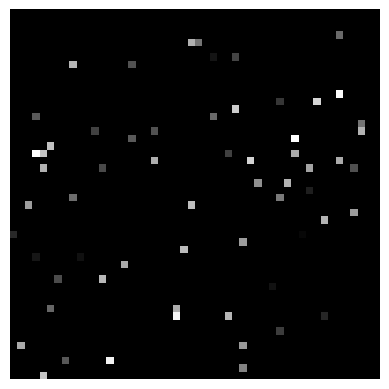
\includegraphics[width=2cm]{imgs/cs-x.png}};
                %
                \node at ($(groundtruth)+(0,-3)$) {$\pdim$ pixels};
            }
            %
            %
            %
            \onslide<2-> {
                \node[text width=0.25\linewidth,align=center] (observation) at (4,2.5) {Compressed signal \\ $\obs = \dic\pv \in \kR^{\ddim}$};
                %
                \draw[ultra thick,->] ($(groundtruth.north east)+(0,-0.25)$) .. controls (0,3.25) .. ($(observation.north west)+(0,-0.25)$) node[midway,fill=TolLightWhite,draw,ultra thick,text width=0.35\linewidth,align=center,yshift=-5] {Linear compression};
                %
                \draw ($(observation)+(0,-1.75)$) node {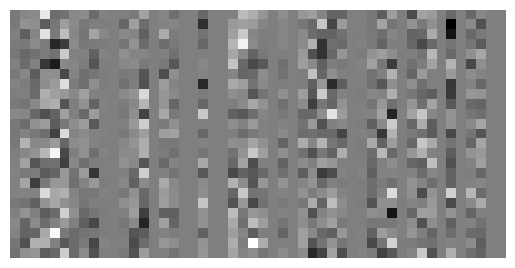
\includegraphics[width=2.5cm]{imgs/cs-y.png}};
                %
                \node at ($(observation)+(0,-2.75)$) {$\ddim$ pixels, $\ddim \ll \pdim$};
            }
            %
            %
            %
            \onslide<3-> {
                \draw[ultra thick,<-] ($(groundtruth.south east)+(0,0.25)$) .. controls (0,1.75) .. ($(observation.south west)+(0,0.25)$) node[midway,fill=TolLightWhite,draw,ultra thick,text width=0.35\linewidth,align=center,yshift=5] {Recover $\pv$ from $\dic$ and $\obs$};
            }
            %
            %
            %
            \onslide<4-> {
                \node [text width=0.45\textwidth] at (0,-1) (problem) {
                    \begin{blockcolor}{mDarkTeal}{Goal}
                    \centering
                    Find $\pv$ such that $\obs = \dic\pv$
                    \end{blockcolor}
                };
            }
            %
            %
            %
            \onslide<5-> {
                \node [text width=0.45\textwidth] at ($(problem)+(0,-2.25)$) (problem-sparse) {
                    \begin{blockcolor}{mDarkTeal}{Goal}
                        \centering
                        Find $\pv$ \textcolor{TolLightOrange}{sparse} such that $\obs = \dic\pv$
                    \end{blockcolor}
                };
                %
                \draw[ultra thick,->] ($(problem)+(0,-0.75)$) -- ($(problem-sparse)+(0,0.5)$) node[midway,fill=TolLightWhite,draw,ultra thick] {no unique solution};
            }
        \end{scope}
    \end{tikzpicture}
\end{frame}
  
\begin{frame}{Feature selection}
    \begin{tikzpicture}[remember picture,overlay]
        \begin{scope}[xshift=0.5\textwidth]
            \onslide<1-> {
                \node (table) at (0,1.5) {
                    \begin{tabular}{c|cccc|c}
                        \toprule
                        & \textbf{Feature 1} & \textbf{Feature 2} & $\quad$...$\quad$ & \textbf{Feature n} & $\ \ $\textbf{Target}$\ \ $ \\
                        \midrule
                        \textbf{Sample 1} & \textcolor{mDarkTeal!20}{$a_{1,1}$} & \textcolor{mDarkTeal!20}{$a_{1,2}$} & \textcolor{mDarkTeal!20}{...} & \textcolor{mDarkTeal!20}{$a_{1,\pdim}$} & \textcolor{mDarkTeal!20}{$\obsi{1}$} \\
                        \textbf{Sample 2} & \textcolor{mDarkTeal!20}{$a_{2,1}$} & \textcolor{mDarkTeal!20}{$a_{2,2}$} & \textcolor{mDarkTeal!20}{...} & \textcolor{mDarkTeal!20}{$a_{2,\pdim}$} & \textcolor{mDarkTeal!20}{$\obsi{2}$} \\
                        \textbf{Sample 3} & \textcolor{mDarkTeal!20}{$a_{3,1}$} & \textcolor{mDarkTeal!20}{$a_{3,2}$} & \textcolor{mDarkTeal!20}{...} & \textcolor{mDarkTeal!20}{$a_{3,\pdim}$} & \textcolor{mDarkTeal!20}{$\obsi{3}$} \\
                        \textcolor{mDarkTeal!20}{...} & \textcolor{mDarkTeal!20}{...} & \textcolor{mDarkTeal!20}{...} & \textcolor{mDarkTeal!20}{...} & \textcolor{mDarkTeal!20}{...} & \textcolor{mDarkTeal!20}{...} \\
                        \textbf{Sample m} & \textcolor{mDarkTeal!20}{$a_{\ddim,1}$} & \textcolor{mDarkTeal!20}{$a_{\ddim,2}$} & \textcolor{mDarkTeal!20}{...} & \textcolor{mDarkTeal!20}{$a_{\ddim,\pdim}$} & \textcolor{mDarkTeal!20}{$\obsi{\ddim}$} \\
                        \bottomrule
                    \end{tabular}
                };
                %
                \node[draw,ultra thick,fill=TolLightWhite,font=\small] (features) at ($(table.center)+(0,-0.5)$) {$\dic \in \kR^{\ddim\times\pdim}$};
                \node[draw,ultra thick,fill=TolLightWhite,font=\small] (outcome) at ($(table.center)+(4.2,-0.5)$) {$\obs \in \kR^{\ddim}$};
            }
            %
            %
            %
            \onslide<2-> {
                \node[text width=0.275\linewidth,align=center] (feature) at ($(table.south)+(-3.5,-0.6)$) {Features $\dic \in \kR^{\ddim\times\pdim}$};
                \node[text width=0.275\linewidth,align=center] (outcome) at ($(table.south)+(3.5,-0.6)$) {Target $\obs = \phi(\dic\pv)$};
                %
                \draw[ultra thick,<->] (feature) -- (outcome) node[midway,below,TolLightOrange] {weights $\pv \in \kR^{\pdim}$};
            }
            %
            %
            %
            \onslide<3-> {
                \node[font=\small,text width=0.3\linewidth,align=center] (loss) at ($(table.south)+(-1.75,-2)$) {\textbf{Model accuracy} \\ Loss $\mathcal{L}_{\phi}(\dic\pv,\obs)$};
                %
                \node[font=\small,text width=0.3\linewidth,align=center] (reg) at ($(table.south)+(1.75,-2)$) {\textbf{Model explainability} \\ Use few features};
            }
            %
            %
            %
            \onslide<4-> {
                \draw[ultra thick,->] (loss) -- ($(loss)+(0,-0.75)$);
                \draw[ultra thick,->] (reg) -- ($(reg)+(0,-0.75)$);
                %
                \node[align=center,text width=0.6\textwidth] (serm) at ($(table.south)+(0,-3.25)$) {
                    \begin{blockcolor}{mDarkTeal}{Goal}
                    \centering
                    Find $\pv$ \textcolor{TolLightOrange}{sparse} such that $\mathcal{L}_{\phi}(\dic\pv,\obs)$ is small 
                    \end{blockcolor}
                };
            }
        \end{scope}
    \end{tikzpicture}
\end{frame}
  
\begin{frame}{Network design}
    \begin{tikzpicture}[remember picture,overlay]
        \begin{scope}[xshift=0.5\textwidth]
            \onslide<1-> {
                \coordinate (A) at (-3.5,1);
                \coordinate (B) at ($(A)+(2,0)$);
                \coordinate (C) at ($(A)+(1,2)$);
                \coordinate (D) at ($(A)+(1,-2)$);
                \coordinate (E) at ($(A)+(3,1)$);
                \coordinate (F) at ($(A)+(3,-1)$);
                \coordinate (G) at ($(A)+(-1,1.5)$);
                \coordinate (H) at ($(A)+(-1,-1.5)$);
                \coordinate (I) at ($(A)+(4,0)$);
                \coordinate (J) at ($(A)+(-2,0)$);

                \draw[ultra thick,dashed] (A) -- (B);
                \draw[ultra thick,dashed] (A) -- (C);
                \draw[ultra thick,dashed] (A) -- (D);
                \draw[ultra thick,dashed] (A) -- (G);
                \draw[ultra thick,dashed] (A) -- (H);
                \draw[ultra thick,dashed] (B) -- (C);
                \draw[ultra thick,dashed] (B) -- (D);
                \draw[ultra thick,dashed] (B) -- (E);
                \draw[ultra thick,dashed] (B) -- (F);
                \draw[ultra thick,dashed] (B) -- (I);
                \draw[ultra thick,dashed] (C) -- (E);
                \draw[ultra thick,dashed] (C) -- (G);
                \draw[ultra thick,dashed] (D) -- (F);
                \draw[ultra thick,dashed] (D) -- (H);
                \draw[ultra thick,dashed] (E) -- (I);
                \draw[ultra thick,dashed] (F) -- (I);
                \draw[ultra thick,dashed] (G) -- (H);
                \draw[ultra thick,dashed] (G) -- (J);
                \draw[ultra thick,dashed] (H) -- (J);

                \node[ultra thick, circle, draw, minimum size=6mm, fill=TolLightWhite] at (A) {};
                \node[ultra thick, circle, draw, minimum size=6mm, fill=TolLightWhite] at (B) {};
                \node[ultra thick, circle, draw, minimum size=6mm, TolLightRed, fill=TolLightWhite] at (C) {\small\textcolor{TolLightRed}{\textbf{3}}};
                \node[ultra thick, circle, draw, minimum size=6mm, TolLightRed, fill=TolLightWhite] at (D) {\small\textcolor{TolLightRed}{\textbf{3}}};
                \node[ultra thick, circle, draw, minimum size=6mm, fill=TolLightWhite] at (E) {};
                \node[ultra thick, circle, draw, minimum size=6mm, fill=TolLightWhite] at (F) {};
                \node[ultra thick, circle, draw, minimum size=6mm, fill=TolLightWhite] at (G) {};
                \node[ultra thick, circle, draw, minimum size=6mm, fill=TolLightWhite] at (H) {};
                \node[ultra thick, circle, draw, minimum size=6mm, TolLightRed, fill=TolLightWhite] at (I) {\small\textcolor{TolLightRed}{\textbf{3}}};
                \node[ultra thick, circle, draw, minimum size=6mm, TolLightBlue, fill=TolLightWhite] at (J) {\small\textcolor{TolLightBlue}{\textbf{9}}};

                \node[text width=0.6\linewidth,align=center] at (-2.5,-2) {Which edges to build to transport products from \textcolor{TolLightBlue}{source} to \textcolor{TolLightRed}{sink} nodes ?};
            }
            %
            %
            %
            \onslide<2-> {
                \node[ultra thick, circle, draw, minimum size=6mm, fill=TolLightWhite] (N1) at (2.25,3) {};
                \node[ultra thick, circle, draw, minimum size=6mm, fill=TolLightWhite] (N2) at (4.75,3) {};
                \draw[ultra thick,dashed] (N1) -- (N2) node[midway,above,font=\small] {edge $\idxentry \in I$} node[midway,below,font=\small] {flow $\pvi{\idxentry} \geq 0$};
            }
            %
            %
            %
            \onslide<3-> {
                \node[text width=0.5\linewidth,align=center,anchor=north] at ($(N1)!0.5!(N2)+(0,-0.75)$) {construct edge $\idxentry \in I$ if $\pvi{\idxentry} > 0$ \\ \textcolor{TolLightOrange}{pay construction cost $c$}};
            }
            %
            %
            %
            \onslide<4-> {
                \node[text width=0.4\linewidth,align=center,anchor=north] at ($(N1)!0.5!(N2)+(0,-2.5)$) {\textbf{Question} \\ How to construct the least number of edges to satisfy transportation needs ?};
            }
            %
            %
            %
            \onslide<5-> {
                \node[text width=0.45\linewidth,align=center,anchor=north] at ($(N1)!0.5!(N2)+(0,-5.25)$) {Find $\pv \in \kR^{\card(I)}$ \textcolor{TolLightOrange}{sparse} such that $\mathcal{Q}(\pv)$ $=$ $0$};
                %
                \draw[ultra thick,<->] ($(N1)!0.5!(N2)+(0,-4.5)$) -- ($(N1)!0.5!(N2)+(0,-5.25)$);
            }
        \end{scope}
    \end{tikzpicture}
\end{frame}

\begin{frame}{Balancing solution quality and problem hardness}
    \begin{tikzpicture}[remember picture,overlay]
        \onslide<1-> {
            \begin{scope}[xshift=0.5\textwidth]
                \node (dataset) at (0,2.5) {
                    \scriptsize
                    \begin{tabular}{c|cccccc|c}
                        \multicolumn{8}{c}{\small{Riboflavin dataset - P. Bühlmann \textit{et al.} (2014)}} \\
                        \toprule
                        Colony & AADK & AAPA & ABFA & ABH & ... & ZUR & \textbf{B2 prod.} \\
                        \midrule
                        \#1 & 8.49 & 8.11 & 8.32 & 10.28 & ... & 7.42 & \textbf{-6.64} \\
                        \#2 & 7.29 & 6.39 & 11.32 & 9.42 & ... & 6.99 & \textbf{-5.43} \\
                        ... & ... & ... & ... & ... & ... & ... & ... \\
                        \#71 & 6.85 & 8.27 & 7.98 & 8.04 & ... & 6.65 & \textbf{-7.58} \\
                        \bottomrule
                    \end{tabular}
                };
                %
                \draw[very thick] ($(dataset.south)+(-2.4,0)$) -- ($(dataset.south)+(-2.4,-0.1)$) -- ($(dataset.south)+(2.15,-0.1)$) node[midway,below,font=\small] {4,088 genes} -- ($(dataset.south)+(2.15,0)$);
            \end{scope}
        }
        %
        %
        %
        \onslide<2-> {
            \begin{scope}[xshift=30,yshift=-80]
                \pgfplotscreateplotcyclelist{cycle_quality_hardness}{
                    TolLightBlue, very thick, mark=*, mark options={scale=0.5}\\
                    TolLightBrown, very thick, mark=*, mark options={scale=0.5}\\    
                    TolLightRed, very thick, mark=*, mark options={scale=0.5}\\
                }
                \begin{groupplot}[
                    group style={
                        group size=2 by 1,
                        horizontal sep=0.2\textwidth,
                    },
                    width   = 0.48\textwidth,
                    height  = 0.4\textwidth,
                    xlabel  = \textbf{Number of genes},
                    legend columns=5, 
                    legend style={
                        at={(-0.35,1)},
                        anchor=south,
                        /tikz/every even column/.style = {column sep=5pt},
                        draw=none,
                    },
                    cycle list name=cycle_quality_hardness,
                    mbaseplot,
                    axis line style = ultra thick,
                    major tick style = {ultra thick,color=mDarkTeal},
                    minor tick style={draw=none},
                    xmajorgrids=true,
                    ymajorgrids=true,
                    major grid style={dotted},
                    axis x line=bottom,
                    axis y line=left,
                ]

                    \nextgroupplot[
                        ylabel = \textbf{Model error},
                        ymode=log,
                        ymin=0.09,
                        ymax=1.5,
                    ]
                    \foreach \method in {omp,lasso,el0ps} {
                        \addplot table[x=nnz_grid,y=\method_test_error,col sep=comma]{data/riboflavin_quality.csv};
                    }

                    \nextgroupplot[
                        ymode=log,
                        ylabel = \textbf{Time (sec.)},
                        ytick={0.001,0.01,0.1,1,10,100},
                        ymax=500,
                        ymin=0.0004,
                    ]
                    \foreach \method in {omp,lasso,l0bnb} {
                        \addplot table[x=nnz_grid,y=\method_solve_time,col sep=comma]{data/riboflavin_quality.csv};
                    }

                    \addlegendentry{Omp (heuristic)};
                    \addlegendentry{Lasso (convex problem)};
                    \addlegendentry{$\ell_0$-problem (np-hard problem)};
                \end{groupplot}
            \end{scope}
        }
    \end{tikzpicture}
\end{frame}
